% Options for packages loaded elsewhere
\PassOptionsToPackage{unicode}{hyperref}
\PassOptionsToPackage{hyphens}{url}
%
\documentclass[
  ignorenonframetext,
  aspectratio=169]{beamer}
\usepackage{pgfpages}
\setbeamertemplate{caption}[numbered]
\setbeamertemplate{caption label separator}{: }
\setbeamercolor{caption name}{fg=normal text.fg}
\beamertemplatenavigationsymbolsempty
% Prevent slide breaks in the middle of a paragraph
\widowpenalties 1 10000
\raggedbottom
\setbeamertemplate{part page}{
  \centering
  \begin{beamercolorbox}[sep=16pt,center]{part title}
    \usebeamerfont{part title}\insertpart\par
  \end{beamercolorbox}
}
\setbeamertemplate{section page}{
  \centering
  \begin{beamercolorbox}[sep=12pt,center]{part title}
    \usebeamerfont{section title}\insertsection\par
  \end{beamercolorbox}
}
\setbeamertemplate{subsection page}{
  \centering
  \begin{beamercolorbox}[sep=8pt,center]{part title}
    \usebeamerfont{subsection title}\insertsubsection\par
  \end{beamercolorbox}
}
\AtBeginPart{
  \frame{\partpage}
}
\AtBeginSection{
  \ifbibliography
  \else
    \frame{\sectionpage}
  \fi
}
\AtBeginSubsection{
  \frame{\subsectionpage}
}
\usepackage{amsmath,amssymb}
\usepackage{iftex}
\ifPDFTeX
  \usepackage[T1]{fontenc}
  \usepackage[utf8]{inputenc}
  \usepackage{textcomp} % provide euro and other symbols
\else % if luatex or xetex
  \usepackage{unicode-math} % this also loads fontspec
  \defaultfontfeatures{Scale=MatchLowercase}
  \defaultfontfeatures[\rmfamily]{Ligatures=TeX,Scale=1}
\fi
\usepackage{lmodern}
\usetheme[]{Pittsburgh}
\usecolortheme{beaver}
\usefonttheme{structurebold}
\ifPDFTeX\else
  % xetex/luatex font selection
\fi
% Use upquote if available, for straight quotes in verbatim environments
\IfFileExists{upquote.sty}{\usepackage{upquote}}{}
\IfFileExists{microtype.sty}{% use microtype if available
  \usepackage[]{microtype}
  \UseMicrotypeSet[protrusion]{basicmath} % disable protrusion for tt fonts
}{}
\makeatletter
\@ifundefined{KOMAClassName}{% if non-KOMA class
  \IfFileExists{parskip.sty}{%
    \usepackage{parskip}
  }{% else
    \setlength{\parindent}{0pt}
    \setlength{\parskip}{6pt plus 2pt minus 1pt}}
}{% if KOMA class
  \KOMAoptions{parskip=half}}
\makeatother
\usepackage{xcolor}
\newif\ifbibliography
\usepackage{graphicx}
\makeatletter
\def\maxwidth{\ifdim\Gin@nat@width>\linewidth\linewidth\else\Gin@nat@width\fi}
\def\maxheight{\ifdim\Gin@nat@height>\textheight\textheight\else\Gin@nat@height\fi}
\makeatother
% Scale images if necessary, so that they will not overflow the page
% margins by default, and it is still possible to overwrite the defaults
% using explicit options in \includegraphics[width, height, ...]{}
\setkeys{Gin}{width=\maxwidth,height=\maxheight,keepaspectratio}
% Set default figure placement to htbp
\makeatletter
\def\fps@figure{htbp}
\makeatother
\setlength{\emergencystretch}{3em} % prevent overfull lines
\providecommand{\tightlist}{%
  \setlength{\itemsep}{0pt}\setlength{\parskip}{0pt}}
\setcounter{secnumdepth}{-\maxdimen} % remove section numbering
\setbeamercovered{highly dynamic}
\ifLuaTeX
  \usepackage{selnolig}  % disable illegal ligatures
\fi
\IfFileExists{bookmark.sty}{\usepackage{bookmark}}{\usepackage{hyperref}}
\IfFileExists{xurl.sty}{\usepackage{xurl}}{} % add URL line breaks if available
\urlstyle{same}
\hypersetup{
  pdftitle={Rethinking American Electoral Democracy},
  pdfauthor={Prof.~Jonathan Cervas},
  hidelinks,
  pdfcreator={LaTeX via pandoc}}

\title{Rethinking American Electoral Democracy}
\author{Prof.~Jonathan Cervas}
\date{Updated: February 16, 2023}

\begin{document}
\frame{\titlepage}

\begin{frame}{Rethinking American Electoral Democracy}
\protect\hypertarget{rethinking-american-electoral-democracy}{}
\end{frame}

\begin{frame}{Chapter 1 - Creating a Model Electoral Democracy}
\protect\hypertarget{chapter-1---creating-a-model-electoral-democracy}{}
\end{frame}

\begin{frame}{Positive view of democracy}
\protect\hypertarget{positive-view-of-democracy}{}
-American widely view democracy as a good thing

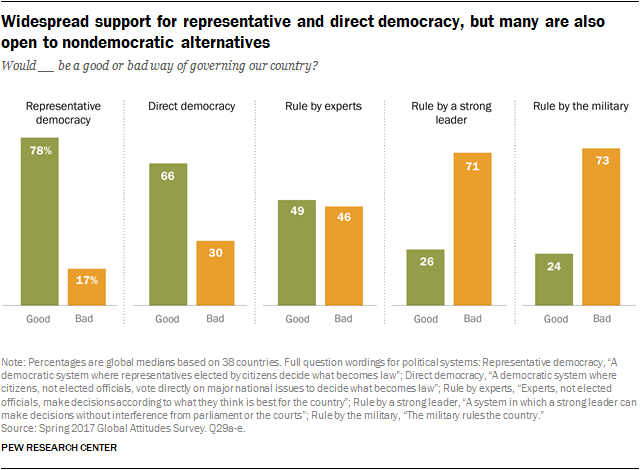
\includegraphics{img/demo-support.png}
\end{frame}

\begin{frame}{Declining trust and confidence}
\protect\hypertarget{declining-trust-and-confidence}{}
\begin{itemize}
\tightlist
\item
  But American's trust and confidence in the wisdom of other Americans
  to make political decisions is in decline
\end{itemize}

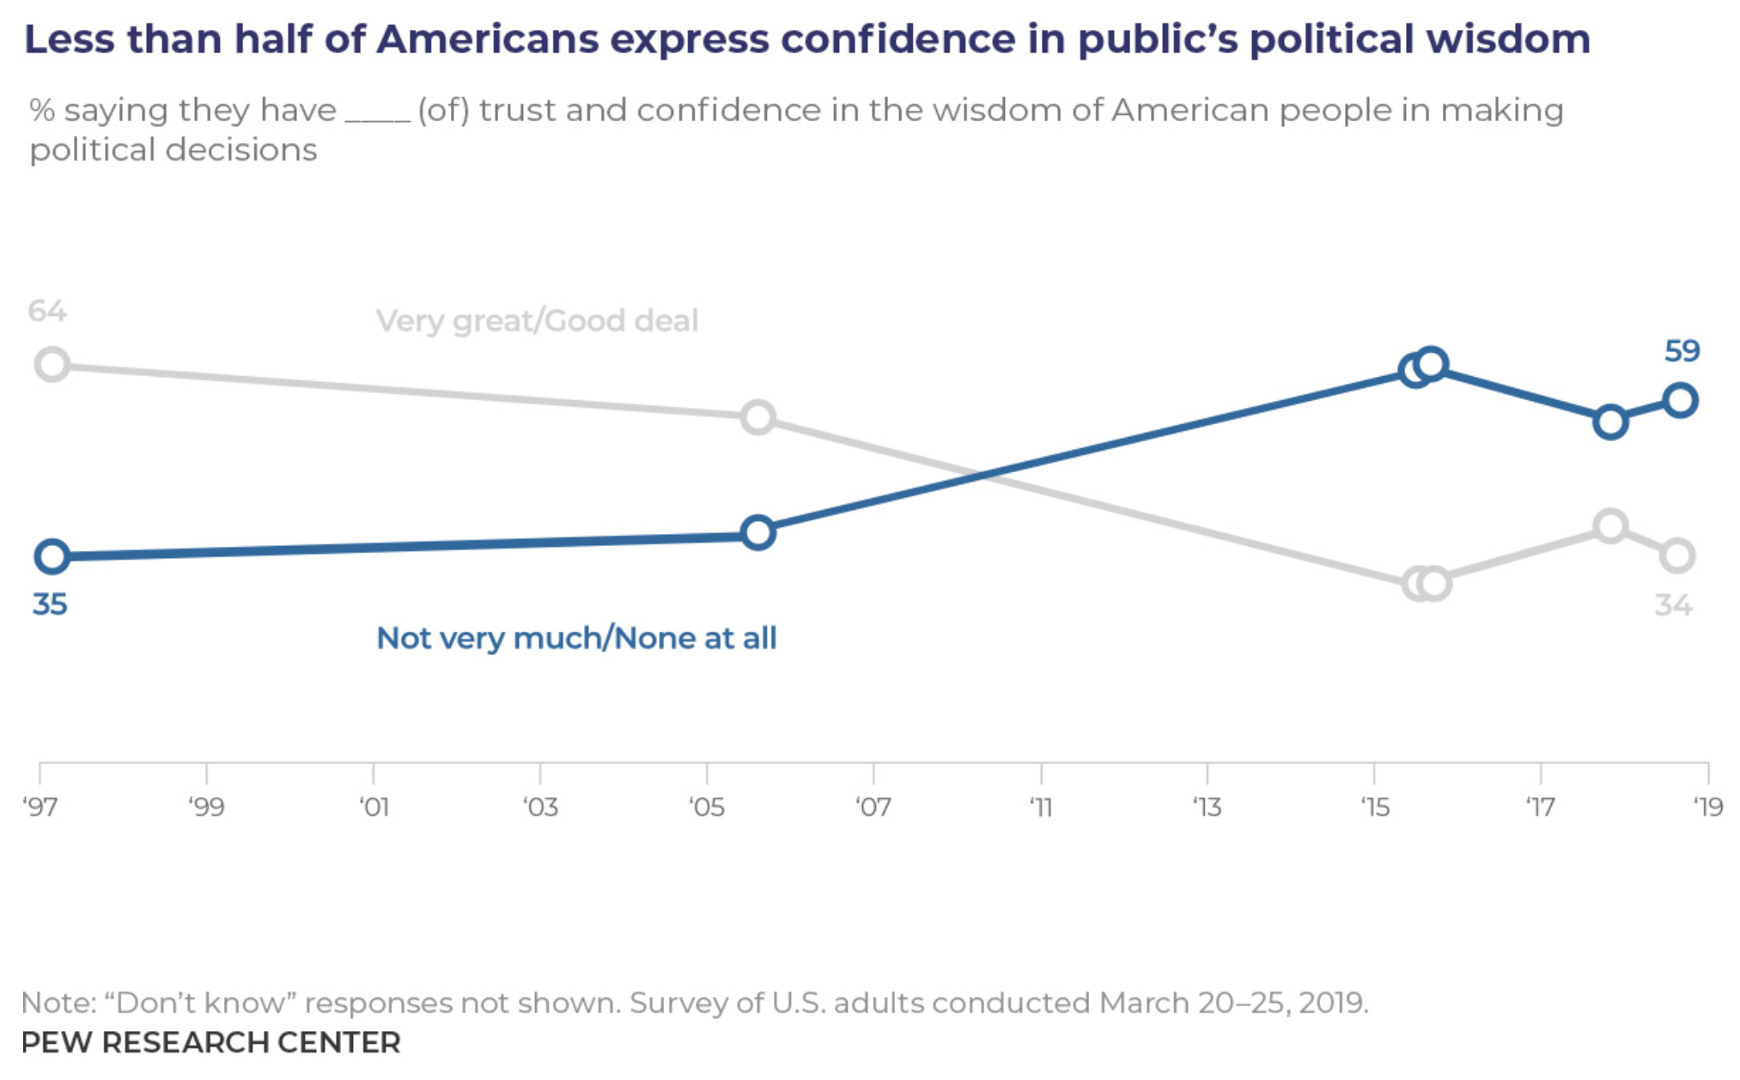
\includegraphics{img/demo-americans.png}
\end{frame}

\begin{frame}{Democracy in trouble?}
\protect\hypertarget{democracy-in-trouble}{}
\begin{itemize}
\tightlist
\item
  A majority (52\%) of young Americans believe that our democracy is
  either ``in trouble,'' or ``failing''\footnote<.->{The Harvard Youth
    Poll, 2,109 18 to 29-year-old U.S. residents conducted between
    Oct.~26 and Nov.~8, 2021.
    \url{https://iop.harvard.edu/youth-poll/fall-2021-harvard-youth-poll}}
\item
  On American Exceptionalism, less than one-third believe that ``America
  is the greatest country in the world''
\item
  Young Americans place the chances that they will see a second civil
  war in their lifetime at 35\%; chances that at least one state secedes
  at 25\%

  \begin{itemize}
  \tightlist
  \item
    Nearly half (46\%) of young Republicans place the chances of a
    second civil war at 50\% or higher, compared to 32\% of Democrats
  \end{itemize}
\end{itemize}
\end{frame}

\begin{frame}{Global Share of the Population living in a democracy}
\protect\hypertarget{global-share-of-the-population-living-in-a-democracy}{}
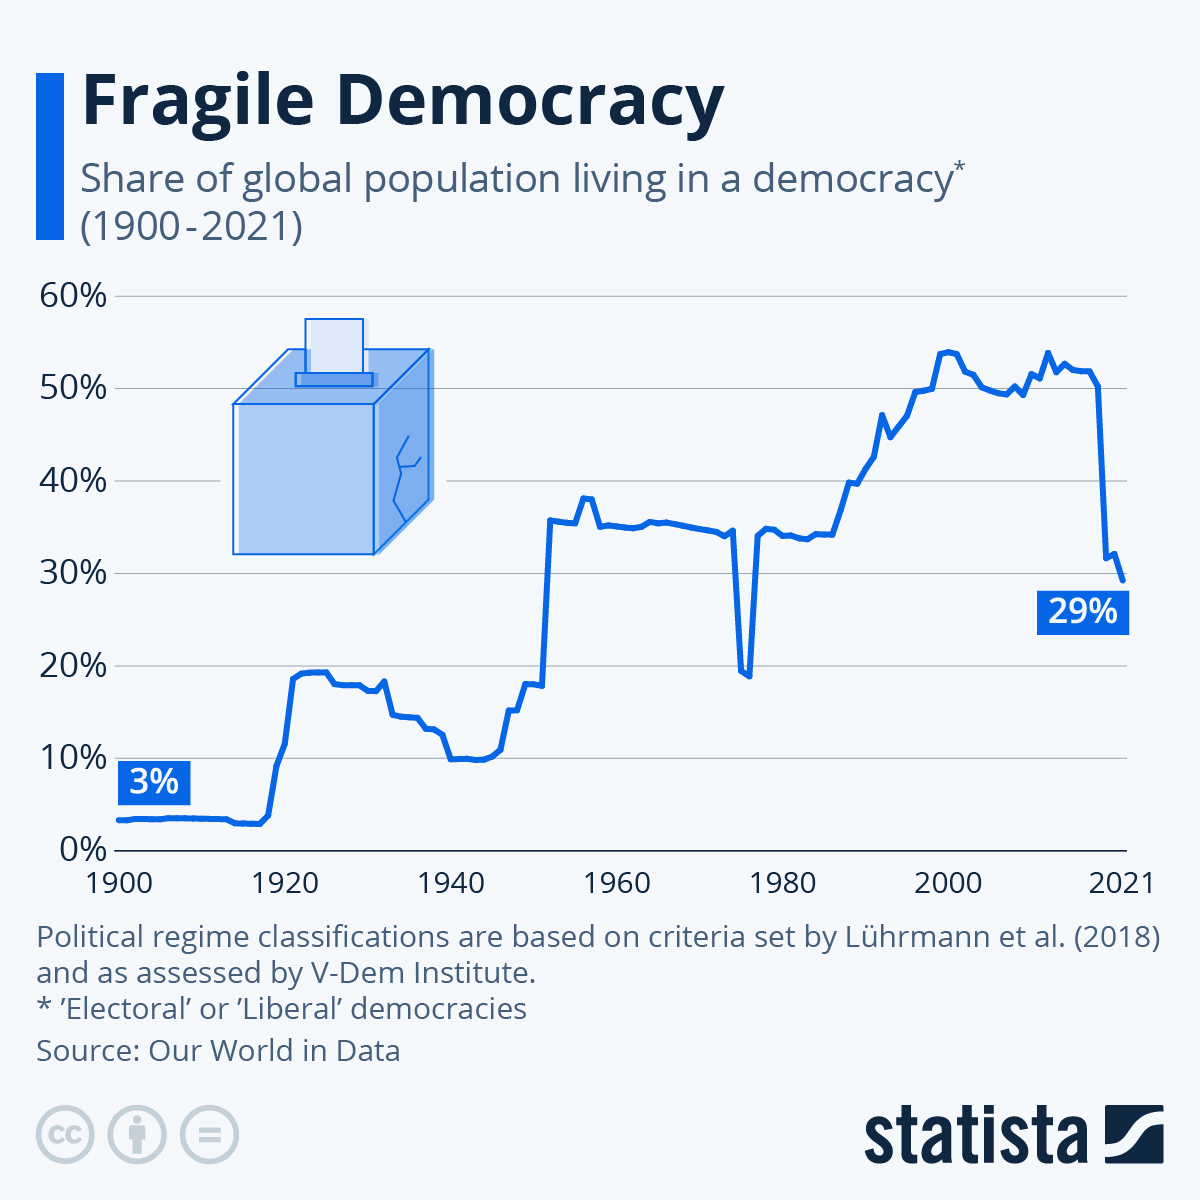
\includegraphics{img/demo-world-pop-share.png}
\end{frame}

\begin{frame}{Public is split on how well democracy is working}
\protect\hypertarget{public-is-split-on-how-well-democracy-is-working}{}
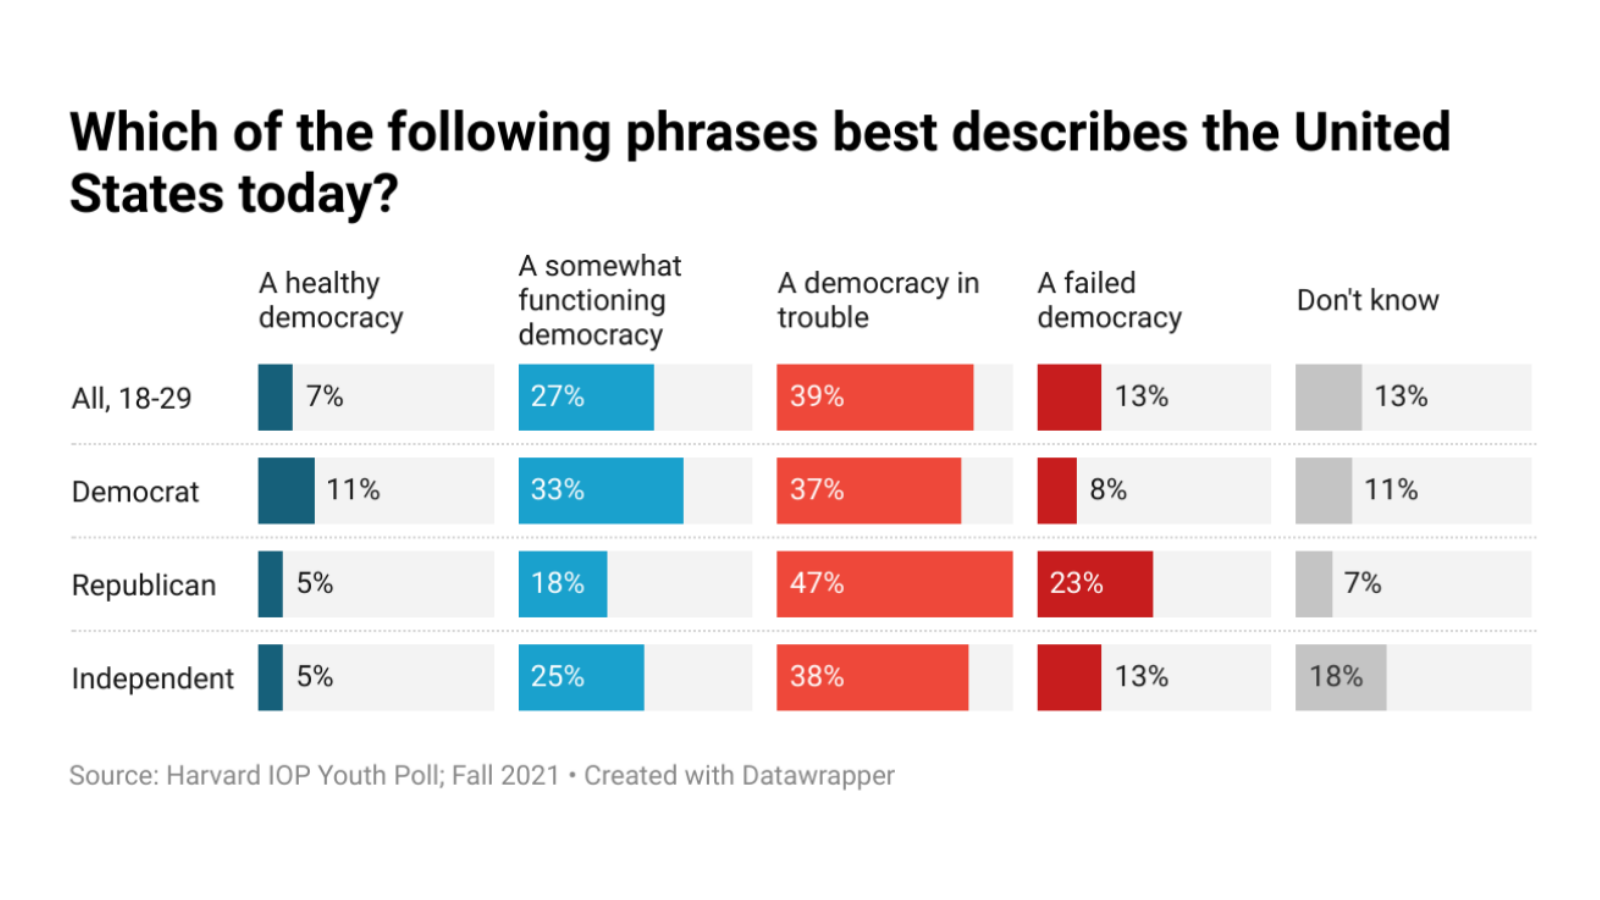
\includegraphics{img/demo-youth.png} \#\#

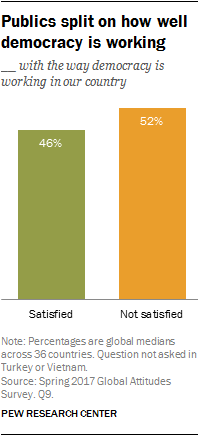
\includegraphics{img/demo-satisfaction.png}
\end{frame}

\begin{frame}{}
\protect\hypertarget{section}{}
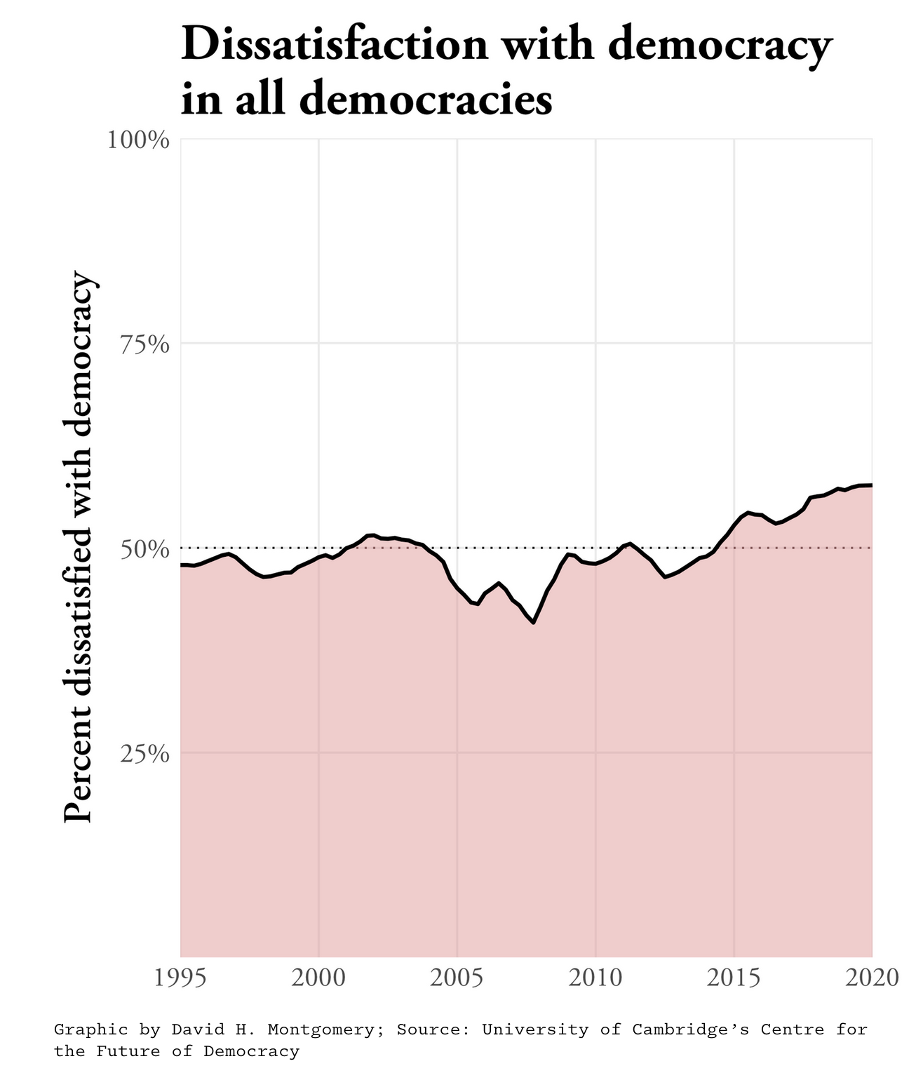
\includegraphics{img/demo-satisfaction-atlantic.png}
\end{frame}

\begin{frame}{}
\protect\hypertarget{section-1}{}
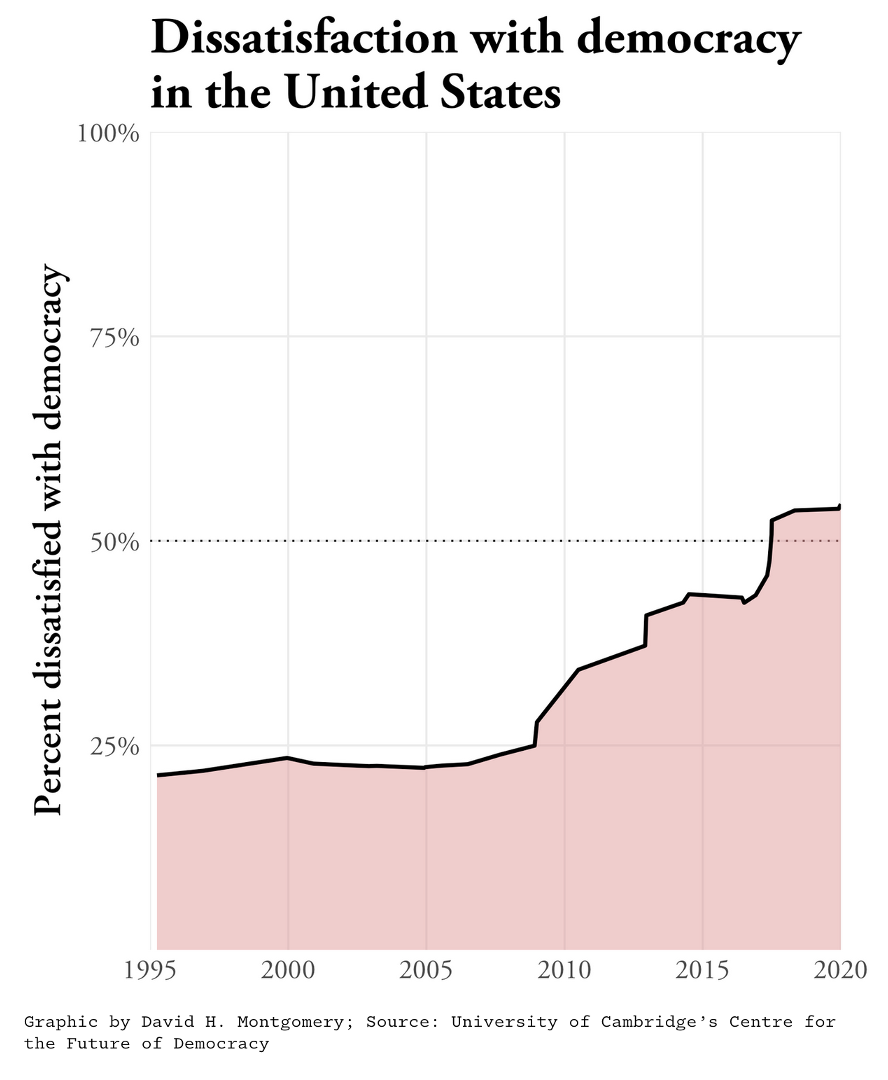
\includegraphics{img/demo-satisfaction-world-atlantic.png}
\end{frame}

\begin{frame}{Basic Facts}
\protect\hypertarget{basic-facts}{}
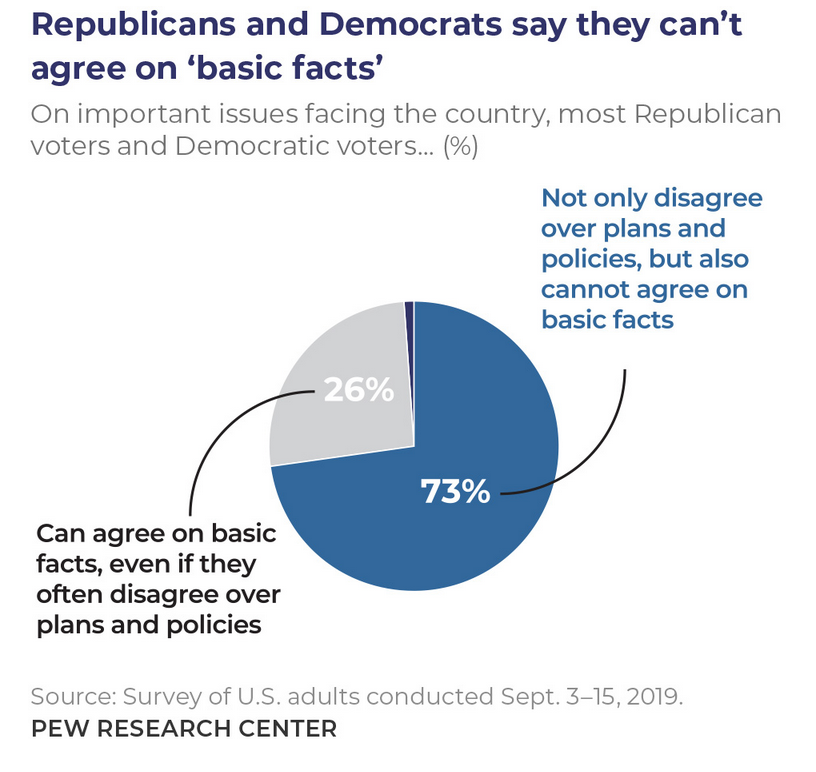
\includegraphics{img/facts-agree.png}
\end{frame}

\begin{frame}{Countries with more democratic systems, greater wealth
show more widespread commitment to representative democracy}
\protect\hypertarget{countries-with-more-democratic-systems-greater-wealth-show-more-widespread-commitment-to-representative-democracy}{}
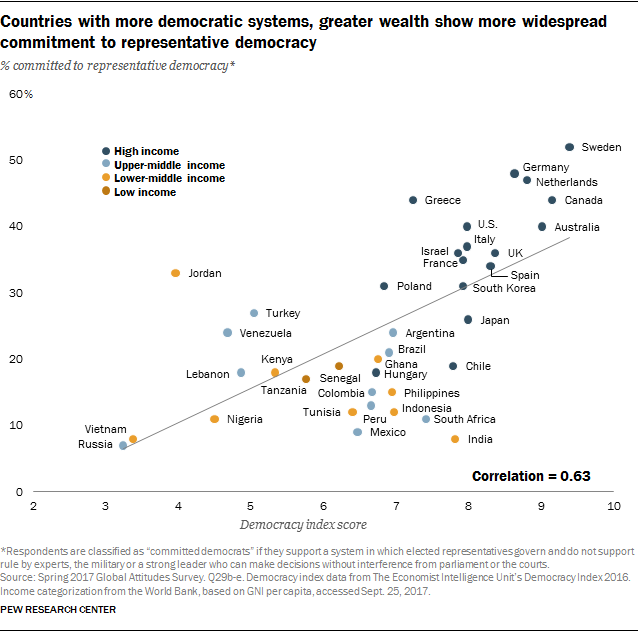
\includegraphics{img/demo-wealth.png}
\end{frame}

\begin{frame}{Assuming Democracy is good\ldots{}}
\protect\hypertarget{assuming-democracy-is-good}{}
\textbf{Assuming democracy is good}:

\begin{itemize}
\item
  How much and what kind of democracy should we have?

  \begin{itemize}
  \item
    Should we have direct democracy where everyone votes on the
    internet?
  \item
    Should this happen for all levels of government, from city issues to
    federal issues?
  \item
    What offices should be elected, and which appointed?
  \item
    Who should appoint, and who should confirm? Can the public recall?
  \end{itemize}
\end{itemize}
\end{frame}

\begin{frame}{Criteria for a Model Electoral Democracy}
\protect\hypertarget{criteria-for-a-model-electoral-democracy}{}
\begin{itemize}
\tightlist
\item
  ``In every democratic country a substantial gap exists between actual
  and ideal democracy. That gap offers us a challenge: can we find ways
  to make `democratic' countries more democratic?''\footnote<.->{Dahl,
    R.A., Dahl, and Yale University Press. 1998. On Democracy. Yale
    University Press.}
\end{itemize}

\begin{itemize}
\tightlist
\item
  One Person, One Vote
\item
  Competitive Elections
\item
  Transparency
\item
  Rules that are not burdensome
\end{itemize}
\end{frame}

\end{document}
